%%%%%%%%%%%%%%%%%%%%%%%%%%%%%%%%%%%%%%%%%%%%%%%%%%%%%%%%%%%%%%%%%%%%%%
% LaTeX Example: Project Report
%
% Source: http://www.howtotex.com
%
% Feel free to distribute this example, but please keep the referral
% to howtotex.com
% Date: March 2011 
% 
%%%%%%%%%%%%%%%%%%%%%%%%%%%%%%%%%%%%%%%%%%%%%%%%%%%%%%%%%%%%%%%%%%%%%%
% How to use writeLaTeX: 
%
% You edit the source code here on the left, and the preview on the
% right shows you the result within a few seconds.
%
% Bookmark this page and share the URL with your co-authors. They can
% edit at the same time!
%
% You can upload figures, bibliographies, custom classes and
% styles using the files menu.
%
% If you're new to LaTeX, the wikibook is a great place to start:
% http://en.wikibooks.org/wiki/LaTeX
%
%%%%%%%%%%%%%%%%%%%%%%%%%%%%%%%%%%%%%%%%%%%%%%%%%%%%%%%%%%%%%%%%%%%%%%
% Edit the title below to update the display in My Documents
%\title{Project Report}
%
%%% Preamble
\documentclass[paper=a4, fontsize=11pt]{scrartcl}
\usepackage{hyperref}

\usepackage[T1]{fontenc}
\usepackage{fourier}
\usepackage{times}
\usepackage{listings}
\usepackage{filecontents}

\usepackage[english]{babel}															% English language/hyphenation
\usepackage[protrusion=true,expansion=true]{microtype}	
\usepackage{amsmath,amsfonts,amsthm} % Math packages
\usepackage[pdftex]{graphicx}	
\usepackage{url}
 \usepackage[top=0.5in, bottom=0.5in, left=1in, right=1in]{geometry}
%%% Custom sectioning
\usepackage{sectsty}
\allsectionsfont{\centering \normalfont\scshape}


%%% Custom headers/footers (fancyhdr package)
\usepackage{fancyhdr}
\pagestyle{fancyplain}
\fancyhead{}											% No page header
\fancyfoot[L]{}											% Empty 
\fancyfoot[C]{}											% Empty
\fancyfoot[R]{\thepage}									% Pagenumbering
\renewcommand{\headrulewidth}{0pt}			% Remove header underlines
\renewcommand{\footrulewidth}{0pt}				% Remove footer underlines
\setlength{\headheight}{13.6pt}

%%% Equation and float numbering
\numberwithin{equation}{section}		% Equationnumbering: section.eq#
\numberwithin{figure}{section}			% Figurenumbering: section.fig#
\numberwithin{table}{section}				% Tablenumbering: section.tab#


%%% Maketitle metadata
\newcommand{\horrule}[1]{\rule{\linewidth}{#1}} 	% Horizontal rule

\title{
		%\vspace{-1in} 	
		\usefont{OT1}{bch}{b}{n}
		\normalfont \normalsize \textsc{Department of Computer Science, Technische Universit\"at Kaiserslautern\\
Compilers and Language Processing Tools - SS17
		} \\ [2pt]
		\horrule{0.5pt} \\[0.4cm]
		\huge A Translator for OO-Constructs\\
		From Minijava to $\mu$-LLVM
		\horrule{2pt} \\[0.5cm]
}

\author{	
		\textbf{Exercise 5}\\
		Group 03\\
        Daniele Gadler, Gopal Praveen\\Alka Scaria, Stephen Banin Payin \\[-1pt]		\normalsize
}


\date{July 2, 2017}

%%% Begin document
\begin{document}
\maketitle

\section*{Overview}
In this report, we describe our group's translator for Object-Oriented constructs from Minijava to $\mu$-LLVM. The resulting Translator successfully converts classes into \textit{TypeStructs}, storing fields of base classes and parents' classes through the usage of replication for supporting inheritance. Furthermore, methods are supported through the creation of a Virtual Method Table per class, where methods of the base class, along with the ones inherited from parent classes, are stored. Inheritance and overriding of methods in classes is hence supported through this virtual method table, which is stored as first field of the \textit{TypeStruct} of the corresponding class. New Objects' instantiation, along with fields' access on the left and right-hand side of an assignment operation is also supported. Methods are translated into global procedures and output in $\mu$-LLVM code, however, the team did not manage to make procedure calls function in $\mu$-LLVM because of problems with referencing the calling object in procedures. 


\section*{Functionalities}
\begin{itemize}
	\item \textbf{Class' Fields to StructFieldList in TypeStruct}: A Class is translated into a \textit{TypeStruct}, containing a \textit{StructFieldList}, where all the different fields accessible in a class are stored. In order to allow fields from parent classes to be accessible through children classes, the layout of parents was made compatible with the one of children. Figure \ref{classes_fields} shows the TypeStructs generated from two Java classes A and B, where class B extends class A. These classes contain respectively fields x and y (A) and y (B). Hence, the TypeStruct for B contains all fields of A according to the principles of \textit{replication}.
	
	\begin{figure}
		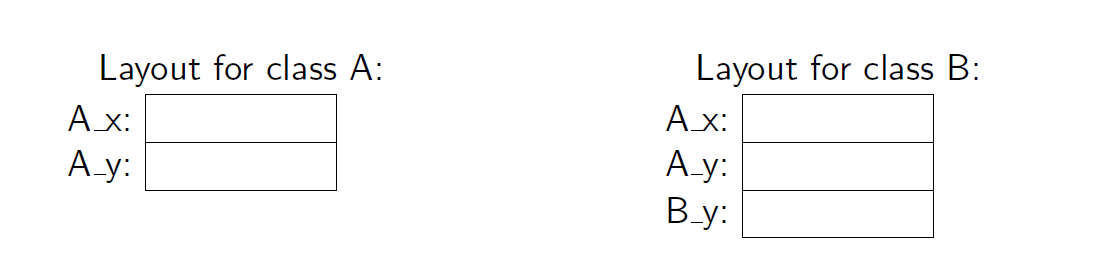
\includegraphics[width=0.75\textwidth]{classes_layout.png}	
		\caption{Compatible TypeStructs' fields layout for supporting inheritance of fields.}
		\label{classes_fields}

	\end{figure}
	
	
	\item \textbf{Class' Methods to Procedures in Virtual Method Table}: All methods contained in a class are translated into procedures, which are stored into a \textit{Virtual Method Table}. A Virtual Method Table is a particular TypeStruct that contains pointers to all the different procedures addressable in a certain class. Furthermore, in order to allow referencing of Virtual Method Tables and the procedures therein contained, these are stored as global variables in the program. Every class declaration has its own Virtual Method Table, which is stored as first field of the class' TypeStruct, as shown Figure \ref{vtable}. It is also worth noting that the layout of Virtual Method Tables was designed so as to support inheritance and overriding among classes' methods. For example, if a base class A contains function f() and extends class B, which also contains a function f(), then the method f() in A is considered to be overriding method f() in B and a single procedure reference to f() is stored both in A's and B's Virtual Method Tables. 

	
	\begin{figure}[h]
		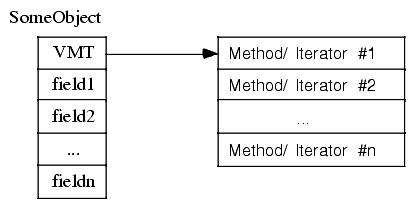
\includegraphics[width=0.8\textwidth]{VTable.png}	
		\caption{Location of the Virtual Method Table inside a Class' Type Struct}
		\label{vtable}

	\end{figure}
	
		\item \textbf{Object instantiation}:  Upon initialization of an object, all fields of the object are initialized to their default value( int --> 0, boolean --> false, int[] and Class --> null): the class' type of the variable the class is being assigned to is checked as well. (For example: A a = new B(), where B extends class A). Should classes on the right-hand and the left-hand side not have the same type, then a Bitcast operation takes place and the left-hand side's type is converted to the right-hand side's type. 

	\item \textbf{Field Access}: Should a Field Access take place on the left or right-hand side of an expression, then respectively a value or a reference to the value store inside the field being accessed is returned. Field accessing is done by retrieving the Object's address on the heap and shifting the pointer's offset by an amount equal to the index of the field (starting from index 1, as the Virtual Method Table is stored at index 0). Since fields are stored together with their class name in the class' TypeStruct, then their name is unique (EX: class A has field x --> Field has name A\_x \ref{classes_fields}). Consequently, lookup of the correct field is performed by matching through the following string for an occurrence in the class' TypeStruct.
	\begin{center}
Field\_Name = ClassName + "\_" + FieldName
\end{center}	

\item \textbf{Procedures and Procedures Calls}: Methods are correctly translated into procedures, along with their body, arguments and return type. When calling a procedure, a reference to the "this" object where the method gets called onto, also needs to be stored into the procedure itself. For this reason, a class reference to that the method is called is stored into the procedure as first argument. Afterwards, a procedure call will need to pass the proper object reference in order for the procedure to access the right class-level fields. Although this may sound good in theory, despite our efforts, all our attempts at implementing procedure calls failed. This is the reason why most test cases are not passing either.  Examples of test cases passing are stored in folder "daniele\_test\_cases" through. 
\item \textbf{Theory}: See folder "Theory".
	

	
\end{itemize}



\end{document}
